\subsection{Physical Robot Experiments and Baseline Comparison}
\label{subsec:results-baseline-comparison}

To evaluate GaitNet's continuous optimization strategy in
unstructured real-world scenarios, a baseline method is established
utilizing the \textit{Legged Perceptive Stack} \cite{leggedcontrol}.
This state-of-the-art framework employs Nonlinear Model Predictive
Control (NMPC) and Whole-Body Control (WBC) based on OCS2.

A custom physical test environment was constructed mirroring our
simulation benchmark parameters
(\autoref{fig:figure-test-environment}). Hardware experiments were
conducted on a Unitree Go1 quadruped navigating narrow strips of
ground interspersed with gaps. We characterize terrain difficulty
metrics as the percentage of unsteppable terrain (ranging from $0\%$
to $40\%$ gap densities).

We systematically evaluate success rate (completing traversal without
falling), total steps taken, and overall traversal time of the
following methods:
\begin{enumerate}
  \item \textbf{Legged Perceptive Stack:} The state-of-the-art model
    predictive control baseline \cite{leggedcontrol}.
  \item \textbf{GaitNet-Single:} An ablation of GaitNet restricted to
    only one leg in swing phase at any given time.
  \item \textbf{GaitNet-Trot:} An ablation of GaitNet restricted to
    only opposing legs in swing concurrently.
  \item \textbf{GaitNet (Full):} Our proposed unlimited acyclic
    footprint generation model.
\end{enumerate}

\begin{figure}[H]
  \centering
  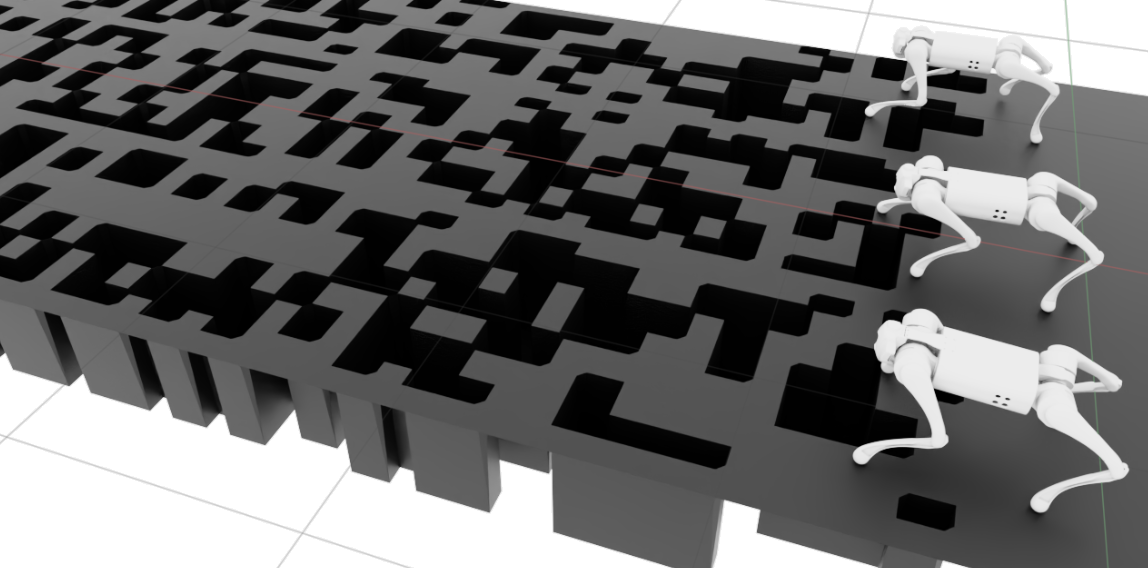
\includegraphics[width=0.8\textwidth]{images/figures/test-environment.png}
  \caption{Unitree Go1 navigating the physical test environment used
    for baseline comparison. The terrain consists of narrow strips
  mapping to varying terrain difficulties (percentage of unsteppable terrain).}
  \label{fig:figure-test-environment}
\end{figure}

GaitNet's unconstrained performance relative to the Legged Perceptive
Stack and fixed-gait ablations reveals a clear advantage in dynamic,
acyclic spatial optimization. The system coordinates multi-leg
motions and adapts continuous spatial timing to minimize total steps
while avoiding invalid terrain. This improvement is particularly
pronounced at higher terrain difficulties ($30$-$40\%$ gap
densities), where restrictive trot strategies inherently clash with
unstructured valid footprints.

\begin{table}[H]
  \centering
  \caption{Placeholder: Real-World Metrics on Unitree Go1}
  \begin{tabular}{lccc}
    \toprule
    \textbf{Method} & \textbf{Success Rate} & \textbf{Avg. Traversal
    Time [s]} & \textbf{Avg. Steps Taken} \\
    \midrule
    Legged Perceptive Stack & XX\% & XX.X & XXX \\
    GaitNet-Single & XX\% & XX.X & XXX \\
    GaitNet-Trot & XX\% & XX.X & XXX \\
    \textbf{GaitNet (Full)} & \textbf{XX\%} & \textbf{XX.X} & \textbf{XXX} \\
    \bottomrule
  \end{tabular}
  \label{tab:hardware-metrics}
\end{table}

\subsection{Simulation Ablations}
\label{subsec:results-simulation-ablations}

In addition to physical trials, simulation ablations were conducted
to validate specific structural choices, notably the swing duration
penalty and action costs within GaitNet. We analyze performance on
similar unstructured tracks but over a more extensive $200$ episode benchmark.

An ablation assessing fixed uniform swing durations versus GaitNet's
dynamic network-predicted durations revealed that the addition of the
duration network head allowed the robot to effectively slow down its
stepping speed over sparse gaps as necessary to maintain equilibrium
while pushing faster transit on solid areas.

Similarly, an action cost penalty of $-0.05$ applied to any
non-no-action choice proved crucial to minimizing jittery or
inefficient consecutive sub-steps. Models evaluated without action
penalties consistently opted for inefficient high-frequency steps
compared to the clean traversal achieved by the penalized model.
GaitNet leverages these continuous penalty variables effectively to
prune excessive locomotion loops and stabilize the quadruped's
spatial gradients.
